% !TEX root = ../../../main.tex
% 所属：第一部分：单变量分析学 / 第1章：实数理论——从Peano公理到实数的连续性
% 节：1.1 朴素集合论
% 正文按原文件顺序保存；由 ../chapter1.tex 调用。
\section{朴素集合论}
我们从朴素集合论开始，这由Cantor建立，在未严格公理化的基础上.请原谅我无法从公理化集合论开始.

\begin{definition}
	集合是具有某种性质的或具体或抽象事物汇集而成的一个整体，这些单一的事物称为集合的元素，用大写字母表示集合，小写字母表示元素.若 $x$ 是 $S$ 的元素则 $x \in S$
	
	我们把以集合为元素的集合称作族，用$\mathcal{A},\mathcal{B},\mathcal{T},\cdots$表示.
\end{definition}

\begin{example}
	集合有两种描述法，列举法和描述法.\\
	$\left\{1\right\},\left\{1,2,3,4\right\}$是列举法；$\left\{x:x>0,x\in\R\right\}$是描述法
\end{example}
\begin{definition}
	空集，是一个不包含任何元素的集合.用 $\varnothing$ 表示
	
\end{definition}
\begin{definition}
	S，T是两个集合，若
	
	\[x \in S \Rightarrow x \in T
	\]
	
	
	也就是说只要 $x \in S$ 就能推出 $x \in T$ .就称 $S$ 是 $T$ 的子集，记为 $S \subset T$
	显然 $x \in S \Rightarrow x \in S$ 故 $S \subset S$
	
\end{definition}
$\varnothing \subset S$ 的证明，用到了逻辑学中的空真原理，我们先对空真原理进行说明
\begin{prp}
	当一个条件语句（如果 P ，那么 Q ）的前提 P 为假，无论Q是真是假，这个条件语句本身必为真.
	

\end{prp}

	\begin{example}
		\begin{enumerate}
			\item 如果 $x$ 是一只独角兽，那么 $x$ 的角是金色的.
			分析：独角兽不存在，故此条件语句中前提是假的、根据空真原理，无法找到一只角不是金色的独角兽来反驳，因此这个条件语句是空真的.
			\item $x\in\R$若$x^2<0$那么$x=23$，这个命题是真的.因为$x\in\R$只能$x^2\geqslant0$.
		\end{enumerate}
\end{example}

这样，我们证明 $\varnothing \subset S$.
根据 $\subset$ 的定义 $\quad x \in \varnothing \Rightarrow x \in S$
,而 $x \in \varnothing$ 假，根据空真原理 $\varnothing\subset S$ 成立.
\begin{definition}
	集合 $S$ ，$T$ 的并，记为 $S \cup T$
	
	$$
	S \cup T=\{x: x \in S \text { 或} x \in T\}
	$$
	
	$S, T$ 的交，记为 $S \cap T$
	
	$$
	S \cap T=\left\{x:x \in S \text { 且 } x \in T\right\}
	$$
	
	$S, T$ 的差，记为 $S \setminus T$
	
	$$
	S\setminus T=\{x :x \in S \text { 且 } x \notin T\}
	$$
	
	$S$ 的补，记为 $S_U^C$ ，$U$ 为全集，有时省略下角标 $U$ ，用 $S^C$ 表示.
	\[S_U^C=\left\{ x:x \in U \text{且} x \notin S\right\}\]
	
	
\end{definition}

\begin{proposition}
	\begin{enumerate}
		\item $A \cup B=B \cup A, A \cap B=B \cap A$ 
		\item$A \cup(B \cup D)=(A \cup B) \cup D, A \cap(B \cap D)=(A \cap B) \cap D$
		\item$A \cap(B \cup D)=(A \cap B) \cup(A \cap D), A \cup(B \cap D)=(A \cup B) \cap(A \cup D)$
	\end{enumerate}

\end{proposition}
\begin{center}
	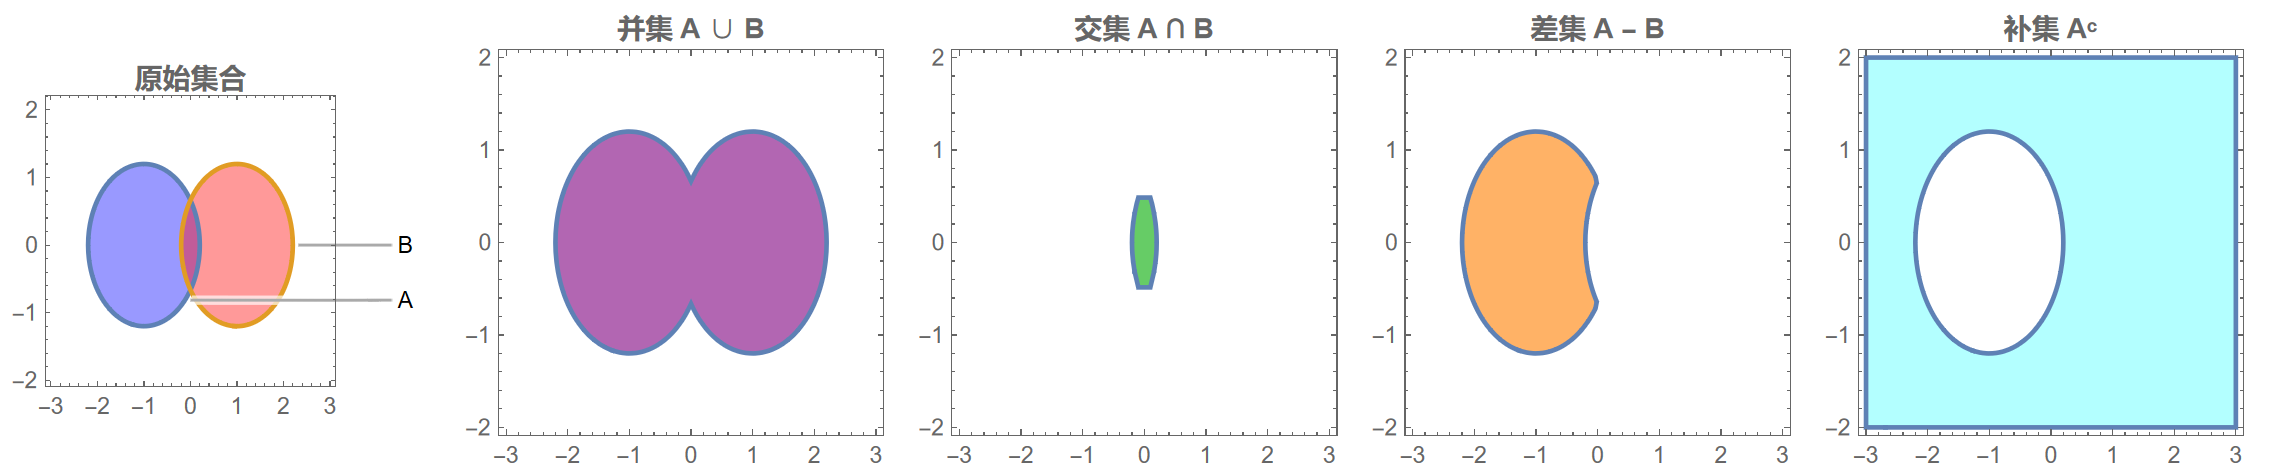
\includegraphics[width=\linewidth]{figure/C1/96aac8f9ecba0c3ccf651dd1b1ab3b43}
	\label{fig:96aac8f9ecba0c3ccf651dd1b1ab3b43}
\end{center}

\begin{proof}
	1，2是显然的，下证3\\
	先证 $A \cap(B \cup D)=(A \cap B) \cup(A \cap D)$
	\\（i）$A \cap(B \cup D) \subset(A \cap B) \cup(A \cap D)$\\
	设 $x \in A \cap(B \cup D) \Rightarrow x \in A$ 并且 $x \in B$ 或 $x \in D \Rightarrow x \in A \cap B$ 或者 $x \in A \cap D \Rightarrow x \in(A \cap B) \cup(A \cap D) \rightarrow A \cap(B \cup D) \subset(A \cap B) \cup(A \cap D)$ \\（ii）$A \cap(B \cup D) \supset( A \cap B) \cup(A \cap D)$\\
	$x \in(A \cap B) \cup(A \cap D) \Rightarrow x \in A$ 且 $x \in B$ 或 $x \in A$ 且 $x \in D \Rightarrow x$ 必 $\in A, x \in B$ 或 $x \in D \Rightarrow x \in A \cap(B \cup D) \rightarrow A \cap(B \cup D) \supset(A \cap B) \cup(A \cap D)$\\故 $A \cap(B \cup D)=(A \cap B) \cup(A \cap D)$
	
	再证 $A \cup(B \cap D)=(A \cup B) \cap(A \cup D)$
	
	$x \in A \cup(B \cap D) \Leftrightarrow x \in A$ 或$x \in B$ 并且 $x \in D \Leftrightarrow x \in A$ 或 $x \in B$ 且 $x \in A$ 或 $x \in D$
	$\Leftrightarrow x \in A \cup B$ 且 $x \in A \cup D \Leftrightarrow x \in(A \cup B) \cap(A \cup D)$
	
	
\end{proof}
\begin{proposition}
	De Morgan 公式
	$$
	(A \cup B)^C=A^C \cap B^C \quad(A \cap B)^C=A^C \cup B^C
	$$
	\label{demordan}
\end{proposition}

\begin{proof}
	先证 $(A \cup B)^C=A^C \cap B^C$
	
	$x \in(A \cup B)^c \Leftrightarrow x \notin A \cup B \Leftrightarrow x \notin A$ 且 $x \notin B \Leftrightarrow x \in A^C$ 且 $x \in B^C \Leftrightarrow x \in A^C \cap B^C$
	
	
	故 $(A \cup B)^c=A^C \cap B^C$
	
	
	
	再证明 $(A \cap B)^C=A^C\cup B^C$
	
	$ x \in(A \cap B)^C \Leftrightarrow x \notin A \cap B \Leftrightarrow x \notin A\text{或}x \notin B \Leftrightarrow x \in A^C\cup B^C$
	
	故 $(A \cap B)^C=A^C \cup B^C$
\end{proof}
\begin{corollary}
	设$\{S_{\alpha}\}$是$M$中的一组集，$\mathcal{A}$是一个指标集，那么
	\[ (\bigcap_{\alpha\in\mathcal{A}}S_{\alpha})^{C}=\bigcup_{\alpha\in\mathcal{A}}S_{\alpha}^{C}\qquad(\bigcup_{\alpha\in\mathcal{A}}S_{\alpha})^{C}=\bigcap_{\alpha\in\mathcal{A}}S_{\alpha}^{C} \]
\end{corollary}
\begin{proposition}
	\begin{enumerate}
		\item $A\setminus\varnothing=A$,$A\setminus  A=\varnothing$
		
		\item$U$是全集，$A\setminus  U=\varnothing$,$U\setminus  A=A^C$
		\item$A\setminus  B=A \cap B^c$
		\item$
		A\setminus  (B \cap C)=(A\setminus  B) \cup(A\setminus  C)
		$
		一般的，有$$X\setminus  \bigcap U_{\alpha}=\bigcup(X\setminus  U_{\alpha})$$
		
		\item$A\setminus  (B \cup C)=(A\setminus  B) \cap(A\setminus  C)$
		一般的，$$X\setminus  \bigcup U_{\alpha}=\bigcap(X\setminus  U_{\alpha})$$
		
		
		\item$A\setminus  B=\varnothing$ 当且仅当 $A \subset B$
		\item 如果 $A \subseteq B$ ，那么对于任意集合 C，有 $A\setminus  C \subseteq B\setminus  C$
		
		如果 $A \subseteq B$ ，那么 $C\setminus  B \subseteq C\setminus  A$
		
	\end{enumerate}
\end{proposition}
\begin{proof}
	\begin{enumerate}
		\item （a）$A\setminus\varnothing=A$
		
		任取 $x$ ， $x \in(A\setminus\varnothing) \Longleftrightarrow(x \in A) \textbf{且}(x \notin \varnothing) \Longleftrightarrow x \in A$ .因为 $x \notin \varnothing$ 恒真.
		所以 $A\setminus \varnothing=A$ .
		
		（b）$A\setminus A=\varnothing$
		
		任取 $x$,
		$
		x \in(A\setminus A) \Longleftrightarrow(x \in A) \textbf{且}(x \notin A) 
		$
		
		
		但 $x \in A$ 与 $x \notin A$ 不可能同时成立，故 $A\setminus A$ 不含任何元素，即 $A\setminus A=\varnothing$ 
		
		\item（a）$A\setminus U=\varnothing$
		
		任取 $x$ ，$x \in(A\setminus U) \Longleftrightarrow(x \in A) \textbf{且}(x \notin U) $
		
		因为 $U$ 是全集，所以 $x \notin U$ 恒假.
		故 $A\setminus U$ 不含任何元素，即 $A\setminus U=\varnothing$ 
		
		（b）$U\setminus A=A^c$
		
		任取 $x$，$x \in(U\setminus A) \Longleftrightarrow(x \in U) \textbf{且}(x \notin A) \Longleftrightarrow \text { True } \textbf{且}(x \notin A) \Longleftrightarrow x \notin A \Longleftrightarrow x \in A^C$
		\item
		
		任取 $x$ ，
		
		$
		x \in(A\setminus B) \Longleftrightarrow(x \in A) \textbf{且}(x \notin B) \Longleftrightarrow(x \in A) \textbf{且}\left(x \in B^C\right) \Longleftrightarrow x \in\left(A \cap B^C\right)
		$
		
		
		所以 $A\setminus B=A \cap B^C$ .
		\item 由3和\ref{demordan}易得
		
		\item 由3和\ref{demordan}易得
		\item
		 $\Rightarrow$ :假设 $A\setminus B=\varnothing$ .要证 $A \subset B$ .
		任取 $x \in A$ .若 $x \notin B$ ，则 $x \in A\setminus B$ ，与 $A\setminus B=\varnothing$ 矛盾.故 $x \in B$ .
		所以 $A \subset B$ .
		
		$\Leftarrow$ :假设 $A \subset B$ .要证 $A\setminus B=\varnothing$ .
		任取 $x \in A\setminus B$ ，则 $x \in A$ 且 $x \notin B$ .但 $A \subset B$ 意味着 $x \in A \Rightarrow x \in B$ ，矛盾.故不存在这样的 $x$ ，即 $A\setminus B=\varnothing$ .
		
		所以 $A\setminus B=\varnothing \Longleftrightarrow A \subset B$ .
		
		\item
		
		（a）如果 $A \subset B$ ，那么对于任意集合 $C$ ，有 $A\setminus C \subset B\setminus C$
		假设 $A \subset B$ .
		任取 $x \in A\setminus C$ ，则 $x \in A$ 且 $x \notin C$ .
		由 $x \in A$ 和 $A \subset B$ 得 $x \in B$ .
		
		所以 $x \in B$ 且 $x \notin C$ ，即 $x \in B\setminus C$ .
		故 $A\setminus C \subset B\setminus C$ .
		
		（b）如果 $A \subset B$ ，那么 $C\setminus B \subset C\setminus A$
		假设 $A \subset B$ .
		任取 $x \in C\setminus B$ ，则 $x \in C$ 且 $x \notin B$ .
		由 $A \subset B$ 和 $x \notin B$ 可得 $x \notin A$（因为若 $x \in A$ 则 $x \in B$ ，矛盾）.
		
		所以 $x \in C$ 且 $x \notin A$ ，即 $x \in C\setminus A$ .
		故 $C\setminus B \subset C\setminus A$ .
	\end{enumerate}
\end{proof}
我们有一下记号
	\[ S=E_1 \cup E_2 \cup \cdots E_n=\bigcup_{x=1}^n E_x\quad \bigcup_{x=1}^{+\infty} E_x\quad \bigcup_{x \in A} E_x \]
	\[T=E_1 \cap E_2 \cap \cdots \cap E_n=\bigcap_{x=1}^n E_x \quad \bigcap_{x=1}^{+\infty} E_x\quad \bigcap_{x \in A} E_x\]	
	
	
这种集合的运算性质，说明了集合构成的类加上交并补的运算可以形成一个代数结构，也就是布尔代数.
\begin{definition}
	对A，B两者的Descartes积定义为
	
	$$
	A \times B:=[(x, y): x \in A, y \in B]
	$$
	
	
	对 $A_1, \cdots, A_n$
	
	$$
	A_1 \times \cdots \times A_n:=\left[\left(x_1, \cdots, x_n\right): x_1 \in A_1, \cdots, x_n \in A_n\right]
	$$
\end{definition}
\newpage
